%% Type de document et encodage de la police
\documentclass[a4paper]{article}
\usepackage[utf8x]{inputenc}

%% Initialise la taille des pages et des marges
\usepackage[a4paper,top=3cm,bottom=3cm,left=2cm,right=2cm,marginparwidth=1.75cm]{geometry}

%% Packs utiles
\usepackage{amsmath}
\usepackage{graphicx}
\usepackage[colorinlistoftodos]{todonotes}
\usepackage[colorlinks=true, allcolors=black]{hyperref}
\usepackage{fourier-orns}
\usepackage{titlesec}
\usepackage{fancyhdr}
\usepackage{fancyvrb}
\usepackage{array}
\usepackage{cancel}
\usepackage{upgreek}
\usepackage{arydshln}
\usepackage{enumerate}

%% Colorbox
\usepackage[most]{tcolorbox}
\usepackage{xcolor}
\definecolor{sprinen}{rgb}{0.0, 1.0, 0.7}

%% Packs utiles pour la manipulation d'image
\usepackage{wallpaper}
\usepackage{amsfonts}
\usepackage{amssymb}
\usepackage{eso-pic}
\usepackage{multicol}
\usepackage{wrapfig}

%% \setlength
\setlength{\parindent}{0.5cm}

%% \thefootnote
\renewcommand{\thefootnote}{\*}
\pagestyle{fancy} 
\setcounter{tocdepth}{5}
\renewcommand{\thefootnote}{\arabic{footnote}}

%% \headrulewidth
\renewcommand{\headrulewidth}{1pt}
\fancyhead[C]{} 
\fancyhead[L]{}
\fancyhead[R]{\footnotesize{\leftmark}}

%% \footrulewidth
\renewcommand{\footrulewidth}{1pt}
\fancyfoot[C]{} 
\fancyhead[L]{}
\fancyfoot[R]{\thepage}

%% definecolor
\definecolor{Zgris}{rgb}{0.87,0.85,0.85}

%% Pour mettre des lignes à gauche et à droite d'un exemple
\usepackage{mdframed}
\newmdenv[
  topline=false,
  bottomline=false,
  skipabove=\topsep,
  skipbelow=\topsep
]{siderules}

%% Redéfinition de la colonne d'un tableau pour que ses éléments soient centrés sur l'axe vertical
%% Implique l'utilisation de \tabularnewline à la place de \\ pour terminer une ligne du tableau
\newcolumntype{M}[1]{>{\raggedright}m{#1}}

%% Pack Tikz pour les diagrammes
\usepackage{tikz}
\usetikzlibrary{shapes.geometric, arrows, shapes, shapes.multipart, decorations.pathmorphing, backgrounds, positioning, fit, petri}
\usetikzlibrary{calc,patterns,decorations.pathmorphing,decorations.markings}
\usetikzlibrary{calc,patterns,decorations.pathreplacing,decorations.markings,3d,backgrounds,tikzmark}

%% Noeuds -> diagrammes
\tikzstyle{rouge} = [rectangle, rounded corners, minimum width = 3cm, minimum height = 1cm, text centered, draw = black, fill = red!30]
\tikzstyle{orange} = [rectangle, minimum width = 3cm, minimum height = 1cm, text
centered, text width = 3cm, draw = black, fill = orange!30]
\tikzstyle{bleu} = [rectangle, minimum width = 3cm, minimum height = 1cm, text
centered, text width = 3cm, draw = black, fill = blue!30]
\tikzstyle{vert} = [diamond, minimum width = 3cm, minimum height = 1cm, text
centered, draw = black, fill = green!30]

%% Pack circuitikz pour les circuits électriques
\usepackage{circuitikz}

%% Utilisation de \mathpzc{}
\DeclareMathAlphabet{\mathpzc}{OT1}{pzc}{m}{it}

%% Pour faire un encadré au coins arrondis
\usepackage{fancybox}
\cornersize{0.25}

%% Pour mettre deux cercles au-dessus d'une lettre \ringring{}
\newcommand\ringring[1]{%
  {% make an Ord atom
   \mathop{\kern0pt #1}\limits^{% set a box over the variable
     \vbox to-1.85ex{
       \kern-2ex % lower the ring accents
       \hbox to 0pt{\hss\normalfont\kern.1em \r{}\kern-.45em \r{}\hss}%
       \vss % fill
     }% end of \vbox
   }% end of the superscript
  }% end of \mathop
}

%% Pour ignorer le itemize
\newcommand\NoIndent[1]{%
  \par\vbox{\parbox[t]{\linewidth}{#1}}%
}









%% Titre, auteur, date
\title{Méthode à la Résolution de Problèmes en Mécanique Rationnelle}
\author{Grégoire Roumache}
\date{Juillet 2018}

\begin{document}

\maketitle

\section{Mouvement du point matériel}





\begin{enumerate}





%% 
\item On commence tous les problèmes de mécanique rationnelle en \textcolor{red}{\textbf{lisant}} attentivement \textcolor{red}{\textbf{l'énoncé}} et en observant le dessin s'il y en a un.





%% 
\item Il faut \textcolor{red}{\textbf{décomposer le mouvement en}} plusieurs \textcolor{red}{\textbf{phases}} si il y a besoin (certains mouvements n'ont qu'une seule phase). Chaque phase correspond à une certaine période de temps et s'étend donc d'un temps $ t_1 $ à un temps $ t_2 $. Quand change-t-on de phase ? Lorsque il y a un changement dans les forces extérieures au système. \\
Exemples : 
\begin{itemize}
\item Dans un premier temps, la fusée expulse du gaz (\textbf{P}) puis arrête ($ \textbf{P} = \textbf{0} $).
\item Un train avance sur des rails ($ \textbf{R}_\nu $) puis déraille ($ \textbf{R}_\nu = \textbf{0} $).
\item Le courant électrique ne passe pas car le circuit est ouvert ($ \textbf{B} = \textbf{0} \implies \textbf{F}_B = \textbf{0} $) puis on le ferme ($ \textbf{B} \neq \textbf{0} \implies \textbf{F}_B \neq \textbf{0} $).
\end{itemize}





%% 
\item On \textcolor{red}{\textbf{liste}} toutes \textcolor{red}{\textbf{les données du problèmes}} qui n'ont "rien" à voir avec les forces et l'accélération. On va donc lister des données comme la masse, la position initiale/intermédiaire/finale, la vitesse ini/inter/fin, les informations en rapport avec le temps, la trajectoire, etc.





%% 
\item Maintenant, on va d'abord \textcolor{red}{\textbf{nommer le}} type de \textcolor{red}{\textbf{mouvement}} (mouvement guidé, chute libre, champ de force/force centrale, particule chargée dans un champ magnétique/électrique, masse variable, ...) puis \textcolor{red}{\textbf{lister}} toutes \textcolor{red}{\textbf{les forces}} selon les trois catégories suivantes : 
\begin{itemize}
\item \textcolor{blue}{\textbf{Force appliquée}} : 
    \begin{itemize}
    \item Gravité : $ \textbf{G} = m \textbf{g} $
    \item Champ de force/force centrale : $\displaystyle \textbf{F} = - \frac{\mu}{s^3} \textbf{s} = - m \mu r^{-2} \textbf{e}_r $
    \item Rappel d'un ressort $ \textbf{F} = - k (l - l_0) \textbf{e} = - k x \textbf{e} = - k \textbf{x} $
    \item Ressort de torsion d'axe $ \textbf{C} = - k (\theta - \theta_0) \textbf{e} = - k \theta \textbf{e} $
    \item Lorentz/électromagnétique $ \textbf{F} = q \; (\textbf{E} + \dot{\textbf{s}} \wedge \textbf{B}) $
    \item Masse variable $\displaystyle \textbf{P} = \frac{d m}{d t} \textbf{v} $
    \end{itemize}
\item \textcolor{blue}{\textbf{Force de liaison}} : 
    \begin{itemize}
    \item Tension dans une corde : proportionnelle à son extension (comme le ressort) seulement lorsque la corde est tendue et étirée.
    \item Force normale : $ \textbf{N} = \textbf{R}_\nu $.
    \item Force binormale : $ \textbf{R}_\beta $.
    \end{itemize}
La force normale est normale à la courbe/surface et la force binormale est une force de réaction normale à la courbe et à \textbf{N}. La binormale est souvent perpendiculaire au plan dans lequel se passe le mouvement.
\item \textcolor{blue}{\textbf{Force de frottement}} : 
    \begin{itemize}
    \item Frottement fluide (loi de Stokes) : $ \textbf{F} = - c \; \dot{\textbf{s}} $
    \item Frottement sec : $\displaystyle \textbf{T} = - \mu N \frac{\dot{\textbf{s}}}{\| \dot{\textbf{s}} \|} $
    \end{itemize}
\end{itemize}
Enfin, on va \textcolor{red}{\textbf{écrire ce qui est en rapport avec l'accélération}}. On note le type d'accélération (centripète, linéaire, ...).





%%
\item Puis on écrit la \textcolor{red}{\textbf{loi de Newton}} (équation différentielle vectorielle du mouvement) : 
\[ \textbf{F} = m \; \ddot{\textbf{s}} \qquad \qquad \qquad \sum \textbf{F}_{\text{extérieures}} = m \; \ddot{\textbf{s}} \]
Si le repère n'est pas inertiel, la loi de Newton s'écrit \footnote{Voir Annexe pour une explication plus détaillée.} : 
\[ \begin{aligned} m \; \textbf{a}_r = m \frac{\delta^2 \textbf{r}}{\delta t^2} &= \textbf{G} - m \; \textbf{a}_e - m \; \textbf{a}_c \\ &= \textbf{G} - m \Big[ \frac{d^2 \textbf{b}}{d t^2} + \dot{\textbf{w}} \wedge \textbf{r} + \textbf{w} \wedge (\textbf{w} \wedge \textbf{r}) \Big] - m \Big[ 2 \textbf{w} \wedge \frac{\delta \textbf{r}}{\delta t} \Big] \end{aligned} \]





%% 
\item Il faut maintenant \textcolor{red}{\textbf{tracer le dessin}}.
\begin{enumerate}
\item Premièrement, on dessine la \textcolor{blue}{\textbf{trajectoire}} du mobile dans l'espace grâce aux données sur sa provenance, sa destination, son type de mouvement (parabolique, circulaire, rectiligne, ...), etc. Il faut aussi placer le mobile sur un point quelconque de sa trajectoire.
\item Deuxièmement, on dessine toutes les \textcolor{blue}{\textbf{forces}} quelles soient appliquées, de liaison ou de frottement. On trace aussi l'\textcolor{blue}{\textbf{accélération}}.
\item Troisièmement, on dessine la \textcolor{blue}{\textbf{vitesse}} et on marque les \textcolor{blue}{\textbf{position initiales et finales}} de la phase de mouvement que l'on étudie.
\end{enumerate}

\end{enumerate}






\begin{center} \textbf{Une fois que l'on a fait ceci, il faut agir en fonction de ce qui est demandé} \end{center}






Ici, on va se retrouver devant plusieurs Questions possible, parmi celles-ci, il y a : 
\begin{enumerate}[A.]
\item L'équation du mouvement est-elle intégrable ?
\item Cherche-t-on la valeur d'un angle, d'un sinus ?
\item Y a-t-il un terme en $ \dot{z}^2 $ dans l'équation de mouvement ?
\item Est-ce un système oscillant ?
\item Est-ce qu'il y a une courbe de guidage mobile ?
\item Doit-on étudier la stabilité du système ?
\end{enumerate}










%% Équation de Newton intégrable
\begin{tcolorbox}[title=A. Équation de Newton intégrable, colback=white, colframe=violet!80, sharp corners]

Si l'équation différentielle du mouvement est linéaire et à coefficients constants, alors elle est résoluble. \\
Solutions de l'équation $\displaystyle a y'' + b y' + c = 0 $ : 
\begin{center} \begin{tabular}{|p{6cm}|p{6cm}|}
\hline
Racines de $ a r^2 + b r + c = 0 $ & Solution générale \\
\hline
$ r_1 $ et $ r_2 $ réelles et distinctes & $\displaystyle y = C_1 e^{r_1 x} + C_2 e^{r_2 x} $ \\
$ r_1 = r_2 = r $ & $\displaystyle y = C_1 e^{r x} + C_2 \; x \; e^{r x} $ \\
$ r_1 $, $ r_2 $ complexes : $ \alpha \pm i \beta $ & $\displaystyle y = e^{\alpha x} (C_1 \cos \beta x + C_2 \sin \beta x) $ \\
\hline
\end{tabular} \end{center}
Et lorsque l'équation différentielle est du type $ a y'' + b y' + c y = G(x) $ : 
\begin{center} \begin{tabular}{|p{6cm}|p{6cm}|}
\hline
$ G(x) $ & À remplacer dans l'équa. diff. \\
\hline
$ G(x) = P(x) $ & $ Y_P = Q(x) $ \\
$ G(x) = e^{k x} P(x) $ & $ Y_P = e^{k x} Q(x) $ \\
$ G(x) = e^{k x} P(x) \cos m x $ & $ Y_P = e^{k x} Q(x) \cos m x + e^{k x} R(x) \sin m x $ \\
\hline
\end{tabular} \end{center}
où $ P(x) $ et $ Q(x) $ sont des polynômes du style de $ a x^2 + b x + c $. \\
Remarques : 
\begin{itemize}
\item $ A \cos m x + B \sin m x = C \cos ( m x + \varphi_1 ) = C \sin ( m x + \varphi_2 ) $.
\item Si $ Y_P(x) $ est une solution de l'équation homogène, alors on remplace $ Y_P(x) $ par $ x Y_P(x) $.
\end{itemize}

\end{tcolorbox}





%% Calcul d'angle, sinus, etc.
\begin{tcolorbox}[title=\textcolor{black}{B. Calcul d'angle ou de trigonométrie}, sharp corners, colback=white, colframe=yellow]

Souvent, si une des étapes consiste à calculer un angle, le sinus d'un angle, etc. On devra projeter l'équation vectorielle de mouvement. Pour faire ceci, on utilise le dessin et on projette chaque force sur les axes adéquats qui sont souvent : la \emph{trajectoire} et la \emph{perpendiculaire à la trajectoire}. \\
Dans le cas où la trajectoire est rectiligne, on projette donc sur cette ligne et sur sa perpendiculaire. Si la trajectoire est, par exemple, circulaire ; on projette sur la tangente à la courbe et sur sa perpendiculaire, la droite joignant la masse et le centre du cercle.

\end{tcolorbox}





%% Présence d'un terme en \dot(z)^2 dans l'équation de mouvement
\begin{tcolorbox}[title=C. Présence d'un terme en $ \dot{z}^2 $ dans l'équation de mouvement, colback=white, colframe=red, sharp corners]

Si la force de frottement est une force divisible par $ \dot{z}^2 $, on utilise la formule $\displaystyle \frac{d^2 z}{d t^2} = \frac{1}{2} \frac{d}{d z} (\dot{z}^2) $ après avoir projeter l'équation vectorielle de mouvement (la formule n'est pas vectorielle). \\
Exemple : $\displaystyle \ddot{z} = g - k \dot{z}^2 $ possède un terme divisible par $ \dot{z}^2 $. En appliquant la formule $\displaystyle \Big( \frac{d^2 z}{d t^2} = \frac{1}{2} \frac{d}{d z} ( \dot{z}^2 ) \Big) $, on obtient : $\displaystyle \frac{1}{2} \frac{d}{d z} (\dot{z}^2) = g - k \dot{z}^2 \implies \frac{d}{d z} (\dot{z}^2) + 2 k \dot{z}^2 - 2 g = 0 $. Dés lors, on pose $ \dot{z}^2 = v^2(z) $, afin de résoudre l'équation différentielle pour la variable $ v^2 $.

\end{tcolorbox}





%% Système oscillant
Dans le cas d'un système oscillant, on va devoir subdiviser le type de système. Il y a : 
\begin{enumerate}
\item L'oscillateur amorti.
\item L'oscillateur avec frottement sec.
\item Les oscillateurs couplés.
\end{enumerate}

\begin{tcolorbox}[title=D. Système oscillant, sharp corners, colback=white, colframe=blue]

Si le système est oscillant, il peut être de trois types : 
\begin{enumerate}
\item L'\textcolor{blue}{\textbf{oscillateur amorti}} est constitué d'une masse, d'un ressort et d'un amortisseur ; son équation de Newton est : $\displaystyle m \ddot{x} = - c \dot{x} - k x $. $\displaystyle \omega_0 = \sqrt{\frac{k}{m}} $ est la fréquence propre du système et $\displaystyle \zeta = \frac{c}{2 \sqrt{k/m}} $ est le facteur d'amortissement du système $ \Big( \ddot{x} + 2 \zeta \omega_0 \dot{x} + \omega_0^2 = 0 \Big) $.
\item L'\textcolor{blue}{\textbf{oscillateur avec frottement sec}}, son équation de Newton est : $\displaystyle m \ddot{x} \textbf{e}_x = (- k x + T) \textbf{e}_x + (N - m g) \textbf{e}_y $. $\displaystyle \omega_0 = \sqrt{\frac{k}{m}} $ est la fréquence propre du système, de sorte que : $\displaystyle \begin{cases} \ddot{x} + \omega_0^2 \; x = - \mu \; g \quad & \text{ si } \dot{x} > 0 \\ \ddot{x} + \omega_0^2 \; x = \mu \; g & \text{ si } \dot{x} < 0 \end{cases} $ \\
Après chaque intervalle de temps $\displaystyle \frac{\pi}{\omega_0} $, l'amplitude de l'oscillation est réduite, si bien que après un moment, la force de friction devient supérieure à la force de rappel du ressort.
\item Les \textcolor{blue}{\textbf{oscillateurs harmoniques couplés}} sont des oscillateurs harmoniques mis en série. Le problème est qu'il y a une relation entre l'élongation des ressorts (la position des masses). Soient $ x_1 $ et $ x_2 $ les axes caractérisant le système. On va étudier les modes propres du système en posant : 
\[ \begin{aligned} X_1 &= x_1 + x_2 \\ X_2 &= x_1 - x_2 \end{aligned} \qquad \qquad \begin{aligned} 2 x_1 &= X_1 + X_2 \\ 2 x_2 &= X_1 - X_2 \end{aligned} \]
où $ X_1 $ et $ X_2 $ sont les modes normaux/propres du systèmes, ils sont normaux car mathématiquement, $ X_1 $ est perpendiculaire à $ X_2 $. \\
On peut étudier séparément la réponse de chacun des modes propres soumis à une force excitatrice\footnote{Exemple en annexe.}.
\end{enumerate}
Remarque : Pour tout système masse-ressort, on place les axes à la longueur naturelle du ressort.

\end{tcolorbox}





%% Courbe de guidage mobile
\begin{tcolorbox}[title=E. Courbe de guidage mobile, colback=white, colframe=orange, rounded corners]

Dans le cas où l'équation différentielle vectorielle de mouvement n'est pas linéaire ou si le mouvement est guidé, on va avoir recours à l'étude de l'intégrale première.
\begin{enumerate}
\item Lorsque la projection sur un axe fixe \textbf{e} de la \emph{résultante} ou du \emph{moment résultant} des forces extérieures appliquées à un système matériel est nulle, on obtient immédiatement une intégrale première du mouvement de ce système.
\begin{align*}
\textbf{e} \cdot \dot{\textbf{N}}_O = \textbf{e} \cdot \textbf{G} &= 0 &&\implies &\textbf{e} \cdot \textbf{N}_O &= \text{ constante } \\
\textbf{e} \cdot \dot{\textbf{H}}_O = \textbf{e} \cdot \textbf{M}_O &= 0 &&\implies &\textbf{e} \cdot \textbf{H}_O &= \text{ constante } \\
\textbf{e} \cdot \dot{\textbf{H}}_C = \textbf{e} \cdot \textbf{M}_C &= 0 &&\implies &\textbf{e} \cdot \textbf{H}_C &= \text{ constante } \\
\end{align*}
\item Lorsque les forces appliquées à un système sont conservatives ou ne développent pas de puissance dans un repère inertiel, il vient : 
\[ \frac{d T_O}{d t} = \mathpzc{P}_O = - \frac{d V}{d t} \qquad \implies \qquad T_O + V = E = \text{ constante } \]
\item Le théorème de l'énergie cinétique est une conséquence directe de la loi de Newton. L'intégrale première de conservation de l'énergie peut donc être obtenue également directement à partir de la loi de Newton. \\
Exemples : 
\begin{itemize}
    \item Glissement sans frottement sur un courbe/surface. \\
    On multiplie l'équation de Newton scalairement par $ \dot{\textbf{s}} $. Et on obtient : 
    \begin{align*} m \ddot{\textbf{s}} &= \textbf{G} + \textbf{R} &m \dot{\textbf{s}} \cdot \ddot{\textbf{s}} &= \dot{\textbf{s}} \cdot (\textbf{G} + \textbf{R}) = \dot{\textbf{s}} \cdot \textbf{G} \end{align*}
    Si les forces données dérivent d'un potentiel, on a : $\displaystyle \dot{\textbf{s}} \cdot \textbf{G} = - \frac{d V}{d t} $. \\
    Et l'intégrale première de conservation de l'énergie : $\displaystyle \frac{1}{2} m \| \dot{\textbf{s}} \|^2 + V = E $. \\
    Cette façon de procéder est assez générale et permet d'obtenir des intégrales premières qui n'apparaissent pas directement par application des théorèmes généraux.

    \item Mouvement d'un point matériel sur une courbe/surface de guidage mobile.
    \begin{align*} m \frac{d^2 \textbf{s}}{d t^2} &= \textbf{G} + \textbf{R} &m \frac{\delta \textbf{s}}{\delta t} \cdot \frac{d^2 \textbf{s}}{d t^2} = \frac{\delta \textbf{s}}{\delta t} \cdot (\textbf{G} + \textbf{R}) &= \frac{\delta \textbf{s}}{\delta t} \cdot \textbf{G} \end{align*}
    Cette fois-ci, on a multiplié l'équation scalairement par la dérivée relative du point par rapport à la courbe/surface. Dans certains cas, cette équation donne lieu à une intégrale première de bilan énergétique. Dans tous les cas, l'intégrale de : $\displaystyle \frac{\delta \textbf{s}}{\delta t} \cdot \textbf{G} $ joue le rôle de potentiel et la constante d'intégration représente une certaine forme de conservation d'énergie du système.
\end{itemize}
\end{enumerate}

\end{tcolorbox}





%% Étude de la stabilité
Pour ce qui est de l'étude de la stabilité, on va agir différemment en fonction de si on a une intégrale première de l'équation du mouvement ou pas.

D'abord, il faut trouver les positions d'équilibre : 

% Positions d'équilibre
\begin{tcolorbox}[title=F. Détermination des positions d'équilibre]
Si on doit trouver les positions d'équilibre d'un système, on pose $ \ddot{x} = 0 $ et $ \dot{x} = 0 $ dans l'équation du mouvement, où \emph{x} est la variable caractéristique du système. Si on a déjà une expression du potentiel $ \big( V(x) \big) $, on peut aussi chercher les valeurs de la variable \emph{x} qui annulent sa dérivée $\displaystyle \Big( V'(x) = \frac{d V(x)}{d x} \Big) $. Ces valeurs sont des positions d'équilibre.
\end{tcolorbox}

% Stabilité - Petites Perturbations
\begin{tcolorbox}[title=\textcolor{black}{G. Étude de la stabilité - Méthode des petites perturbations}, colback=white, colframe=sprinen, sharp corners]

    \begin{tcolorbox}[colback=white,colframe=white,sharp corners,sidebyside,lefthand ratio=0.5]
    Si on a déjà une intégrale première, 
    \begin{enumerate}
        \item Pour trouver les positions d'équilibre, on va annuler la dérivée du potentiel $ \big( V'(x) = 0 \big) $.
        \item On fait un développement de Taylor de : $ V'(x_{\text{eq}} + \eta) $, jusqu'au $ 1^{\text{er}} $ terme non-nul. On le met ensuite dans l'éq. \\ $ m \ddot{\upeta} + V'(x_{\text{eq}} + \upeta) = 0 $ et on obtient : \[ m \ddot{\upeta} + \frac{1}{k !} V^{(k + 1)} (x_{\text{eq}}) \upeta^k \]
        \item On remplace : \[ \mu = \frac{1}{m \; k !} V^{(k + 1)} (x_{\text{eq}}) \]
    \end{enumerate}
    \tcblower
    Si on a pas d'intégrale première à disposition, 
    \begin{enumerate}
        \item On pose $ \ddot{x} = \dot{x} = 0 $ et on annule l'équation de Newton pour trouver les positions d'équilibre.
        \item On fait le développement de Taylor de $ F(x_{\text{eq}} + \upeta) $ jusqu'au 1er terme non-nul dans l'équation de Newton et on obtient : \[ \ddot{\upeta} + \mu \; \upeta^k = 0 \]
        \item On remplace : \[ \frac{1}{2} \dot{\upeta}^2 + \frac{\mu}{k + 1} \upeta^{k + 1} = \text{ constante } \]
    \end{enumerate}
    \end{tcolorbox}

            \begin{tikzpicture}[overlay,remember picture]
                \draw[sprinen,dashed,thick] (8,-0.25) -- (8,8.5);
            \end{tikzpicture}

%% Au-dessus de la ligne
\tcblower
%% En-dessous de la ligne
\begin{center} 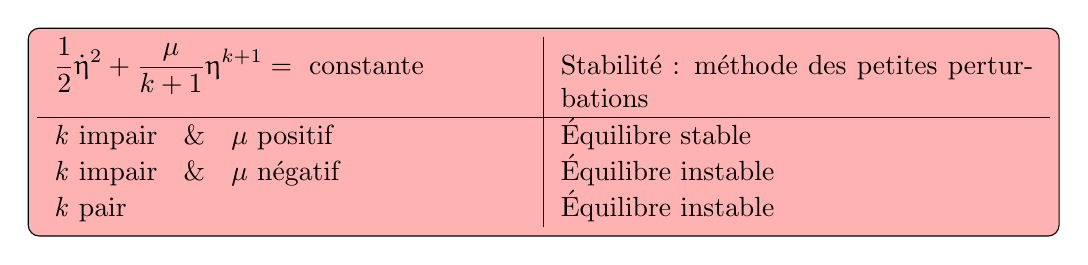
\begin{tikzpicture}
\node (tab) [rouge] {
\begin{tabular}{p{6cm}|p{6cm}}
$\displaystyle \frac{1}{2} \dot{\upeta}^2 + \frac{\mu}{k + 1} \upeta^{k + 1} = \text{ constante } $ & Stabilité : méthode des petites perturbations \\
\hline
\emph{k} impair \; \& \; $ \mu $ positif & Équilibre stable \\
\emph{k} impair \; \& \; $ \mu $ négatif & Équilibre instable \\
\emph{k} pair & Équilibre instable \\
\end{tabular} };
\end{tikzpicture} \end{center}

\end{tcolorbox}





%% Explications pratiques de l'utilisation du diagramme de potentiel
En pratique, on va utiliser le potentiel de la manière suivante : Pour trouver les positions d'équilibre, on peut dériver le potentiel $ \big( \rightarrow V'(x) \big) $ et voir où ça s'annule. \\
Ensuite, on calcule la dérivée seconde pour voir si c'est stable : 
\begin{itemize}
\item $ V''(x) < 0 \longrightarrow $ \; 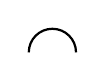
\begin{tikzpicture} \draw [-, thick] (-0.3,2.5) arc (180:0:.3cm); \end{tikzpicture} \; $ [ - x^2 \rightarrow f'' = - 2 ] $
\item $ V''(x) > 0 \longrightarrow $ \; 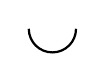
\begin{tikzpicture} \draw [-, thick] (-0.3,2.5) arc (-180:0:.3cm); \end{tikzpicture} \; $ [ + x^2 \rightarrow f'' = + 2 ] $
\item $ V''(x) = 0 \longrightarrow $ Aucune information, il faut encore dériver\footnote{Voir annexe pour voir plus en détail.}.
\end{itemize}
\danger Il faut dériver $ V(x) $ en fonction de \emph{x} $\displaystyle \longrightarrow V'(x) = \frac{d V(x)}{d x} $.





% Stabilité - Perturbations Infinitésimales
\begin{tcolorbox}[title=\textcolor{black}{H. Étude de la stabilité - Méthode des perturbations infinitésimales}, colback=white, colframe=cyan!50, sharp corners]

On va utiliser le développement de Taylor sur l'équation de Newton : $ \ddot{x} + F(x) = 0 $, dans laquelle on introduit : $ x = x_{\text{eq}} + \upeta $. On obtient : \[ \ddot{\upeta} + F'(x_{\text{eq}}) \upeta = 0 \]

\begin{center} \begin{tabular}{|c|c|c|}
\hline &&\\
\textbf{Polynôme caractéristique} & \textbf{Solution générale} & \textbf{Stabilité} \\ && \\
\hline && \\
$ \begin{aligned} z^2 - &\alpha^2 = 0 \\ z_1 = \alpha \; \; &\& \; \; z_2 = - \alpha \end{aligned} $ & $ \begin{aligned} x(t) &= C'_1 e^{\alpha t} + C'_2 e^{- \alpha t} \\ &= C_1 \text{ sh } \alpha t + C_2 \text{ ch } \alpha t \end{aligned} $ & Équilibre instable \\&& \\\hline&& \\
$ \begin{aligned} z^2 + &\alpha^2 = 0 \\ z_1 = i \alpha \; \; &\& \; \; z_2 = - i \alpha \end{aligned} $ & $ \begin{aligned} x(t) &= C'_1 e^{i \alpha t} + C'_2 e^{- i \alpha t} \\ &= C_1 \sin \alpha t + C_2 \cos \alpha t \end{aligned} $ & Équilibre marginalement stable \\&& \\\hline&& \\
$ \begin{aligned} z^2 &= 0 \\ z_1 &= z_2 = 0 \end{aligned} $ & $ x(t) = A t + B $ & Équilibre faiblement instable \\ && \\
\hline
\end{tabular} \end{center}

\end{tcolorbox}






























\newpage





\section{Mouvement du solide}





\subsection{Calcul du centre de masse - tenseur d'inertie}





\begin{enumerate}





\item On commence par préciser le \textcolor{blue}{\textbf{type de système}}, c-à-d sa forme (rectiligne, circulaire, ...) \textcolor{blue}{\textbf{et ses caractéristiques}} telles sa longueur, sa masse, etc. \\
Exemple : "Disque de rayon \emph{R}, de masse \emph{m} et d'épaisseur négligeable".





\item On calcule \textcolor{blue}{\textbf{le centre d'inertie}} qui est le point \emph{C} tel que : $\displaystyle m \textbf{c} = \textbf{Q}_0 = \int_{\text{solide}} \textbf{s} \; d m $. On trouve \emph{C} facilement car il \textcolor{blue}{\textbf{se situe sur l'axe de symétrie du solide}}. On peut aussi utiliser les théorèmes de Guldin : 
\begin{itemize}
    \item Solide = courbe plane homogène : \\
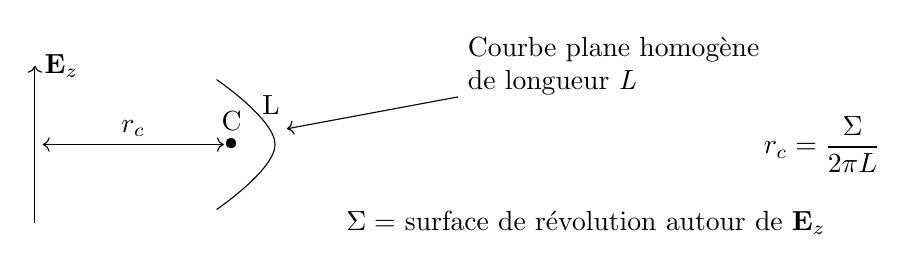
\begin{tikzpicture}
\coordinate (c) at (2.5,0);
\draw [->] (0,-1) -- (0,1) node[right]{$ \textbf{E}_z $};
\node [] at (c) {\textbullet}; \node [yshift=0.3cm] at (c) {C};
\draw [<->] (0.1,0) -- ($ (c) - (0.1,0) $) node[midway, yshift=0.2cm]{$ r_c $};
\draw  plot[smooth, tension=.7, scale=0.55] coordinates {($ (c) - (0.35,1.5) $) ($ (c) + (1,0) $) ($ (c) + (-0.35,1.5) $)};
\node (L) [] at ($ (c) + (0.5,0.5) $) {L};
\node (texte1) [text width=4cm] at ($ (c) + (5,1) $) {Courbe plane homogène de longueur \emph{L}};
\draw [->] (texte1) -- ($ (L) - (-0.2,0.3cm) $);
\node [] at (10,0) {$\displaystyle r_c = \frac{\Sigma}{2 \pi L} $};
\node [] at (7,-1) {$ \Sigma = $ surface de révolution autour de $ \textbf{E}_z $};
\end{tikzpicture}
    \item Solide = surface plane homogène : \\
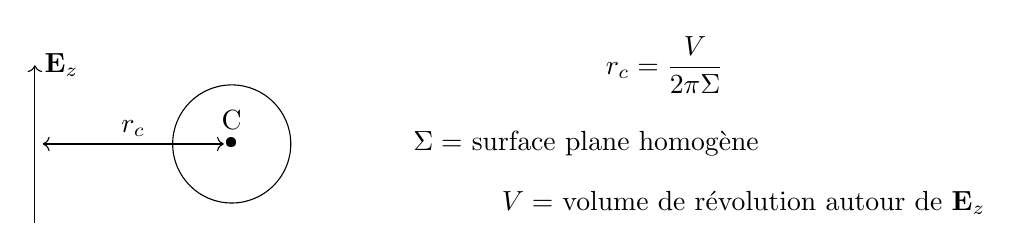
\begin{tikzpicture}
\coordinate (c) at (2.5,0);
\draw [->] (0,-1) -- (0,1) node[right]{$ \textbf{E}_z $};
\node [] at (c) {\textbullet}; \node [yshift=0.3cm] at (c) {C};
\draw [<->] (0.1,0) -- ($ (c) - (0.1,0) $) node[midway, yshift=0.2cm]{$ r_c $};
\draw [black, xshift=2.5cm] circle [radius=0.75cm];
\node [] at (8,1) {$\displaystyle r_c = \frac{V}{2 \pi \Sigma} $};
\node [] at (7,0) {$ \Sigma = $ surface plane homogène};
\node [] at (9,-0.75) {$ V = $ volume de révolution autour de $ \textbf{E}_z $};
\end{tikzpicture}
\end{itemize}





%% Principe de superposition
\item Si le solide est composé de plusieurs parties, on utilise le \textcolor{red}{\textbf{principe de superposition}} : 
\[ m \textbf{c} = m_1 \textbf{c}_1 + m_2 \textbf{c}_2 \]
Et si il y a un "trou" ($ m_2 \textbf{c}_2 $) dans la partie ($ m_1 \textbf{c}_1 $), le principe de superposition devient : 
\[ m \textbf{c} = m_1 \textbf{c}_1 - m_2 \textbf{c}_2 \]





%% Calcul du tenseur d'inertie
\item Maintenant, on calcule le \textbf{tenseur d'inertie} (par rapport à \emph{B}) : 
\[ \textbf{J}_B = \int_{\text{solide}} \Big( s^2 \; \textbf{I} - \textbf{s} \; \textbf{s} \Big) \; d m \]
\[ J_B = \int \begin{pmatrix} y^2 + z^2 & - x y & - x z \\ - x y & x^2 + z^2 & - y z \\ - x z & - y z & x^2 + y^2 \end{pmatrix} \; d m \]
On peut diagonaliser la matrice en l'exprimant dans \textcolor{red}{\textbf{les axes principaux d'inertie}} du solide qui \textcolor{red}{\textbf{correspondent aux éléments de symétrie}} du solide. \\
On fixe le \textcolor{blue}{\textbf{repère au centre d'inertie \emph{C}}} du solide \textcolor{blue}{\textbf{ou}} alors \textcolor{blue}{\textbf{au point \emph{O} si le solide est fixé en ce point}}.
$ J_C = \begin{pmatrix} J_1 & 0 & 0 \\ 0 & J_2 & 0 \\ 0 & 0 & J_3 \end{pmatrix} = \text{ diag } (J_1, J_2, J_3) $ dans la base des a.p.i. (axes principaux d'inertie).
\begin{equation*} \begin{cases} \displaystyle
J_1 = \int \Big( x_2^2 + x_3^2 \Big) \; d m \\ \displaystyle
J_2 = \int \Big( x_1^2 + x_3^2 \Big) \; d m\\ \displaystyle
J_3 = \int \Big( x_1^2 + x_2^2 \Big) \; d m
\end{cases} \end{equation*}
\[ \textbf{J}_C = J_1 \textbf{e}_1 \textbf{e}_1 + J_2 \textbf{e}_2 \textbf{e}_2 + J_3 \textbf{e}_3 \textbf{e}_3 \]





\item Théorèmes particuliers en rapport avec le tenseur d'inertie : 
\begin{itemize}
    \item \textcolor{red}{\textbf{\danger Théorème C}} : 
\[  \textbf{J}_O = \textbf{J}_C + m \; \Big[ c \; \textbf{I} - \textbf{c} \textbf{c} \Big] \]
    \item Moment d'inertie par rapport à une droite \emph{d} de direction \textbf{e} passant par \emph{B} est donné par : 
\[ J_B^d = \textbf{e} \cdot \textbf{J}_B \cdot \textbf{e} \]
où \textbf{e} est unitaire.
    \item Le \textcolor{red}{\textbf{théorème de transport}} est un théorème qui donne le moment d'inertie autour d'une droite $ d_1 $ passant par \emph{O} parallèle à $ d_2 $ passant par \emph{C} : $\displaystyle J_O^{d_1} = J_C^{d_2} + m l^2 $.
\end{itemize}





%% Cas particuliers
\item Cas particuliers : 
\begin{enumerate}
\item[(a)] \textcolor{red}{\textbf{Système rectiligne}} : Il suffit de calculer un seul moment d'inertie par rapport à une droite perpendiculaire à la droite du solide.
\item[(b)] \textcolor{red}{\textbf{Système plan}} : (plan $ Oxy $, $ z = 0 $)
\[ J_x = \int y^2 \; d m \qquad ; \qquad J_y = \int x^2 \; d m \qquad ; \qquad J_z = \int \Big( x^2 + y^2 \Big) \; d m \]
Et donc : $\displaystyle J_x + J_y = J_z \qquad ; \qquad J_{y z} = J_{x z} = 0 $ et l'ellipsoïde d'inertie est donné par : 
\[ J_x x^2 + J_y y^2 + (J_x + J_y) z^2 - 2 J_{x y} x y = 1 \]
Son intersection avec le plan $ Oxy $ ($ z = 0 $) donne l'ellipse d'inertie d'équation : 
\[ J_x x^2 + J_y y^2 - 2 J_{x y} x y = 1 \]
\end{enumerate}





%% Remarque
\item \textbf{Remarque} : Il ne faut jamais utiliser les coordonnées sphérique. Il vaut mieux utiliser les coordonnées sphériques, même pour le calcul sur une sphère\footnote{Voir annexe pour un exemple de calcul du $ \textbf{J}_C $ d'une sphère en coordonnées cylindriques.}.


\end{enumerate}










\section{Étude du mouvement du solide comme vu au cours (!)}





\begin{enumerate}





\item On commence par préciser le \textcolor{orange}{\textbf{type de système}}, c-à-d sa forme (rectiligne, circulaire, ...) \textcolor{orange}{\textbf{et ses caractéristiques}} telles sa longueur, sa masse, etc.

\item On décrit le \textcolor{orange}{\textbf{mouvement du solide}} (mouvement plan, rectiligne, ...) et ses \textcolor{orange}{\textbf{degrés de liberté}} en précisant leur type (translation, rotation, ...), ainsi que les \textcolor{orange}{\textbf{liaisons}}. \\
On en déduit le nombre de variables cinématiques.

\item On donne les \textcolor{orange}{\textbf{systèmes d'axes}} que l'on va utiliser : axes inertiel, axes parallèles aux axes inertiel en \emph{C}, axes principaux d'inertie du solide, coordonnées cylindriques/polaires, etc. \\
Il faut aussi écrire l'équation du \textcolor{orange}{\textbf{vecteur de Poisson}} (ex : $ \boldsymbol{\omega} = ... \; \textbf{E}_z $). \\
On essaie que l'axe $ \textbf{E}_z $ pointe dans la même direction pour tous les repères par soucis de cohérence et éviter les erreurs lors des produits scalaires/vectoriels.

%% Choix des coordonnées généralisées & des repères
\textcolor{red}{\textbf{Remarque}} : Comment choisir le système d'axes approprié ? \\
Pour choisir les coordonnées généralisées et les repères, on commence par : 
\begin{enumerate}
    \item Mettre un \textcolor{orange}{\textbf{repère absolu}} : O, $ \textbf{E}_x $, $ \textbf{E}_y $, $ \textbf{E}_z $.
    \item Si il y a une rotation, placer un repère : \textcolor{orange}{\textbf{$ C_{\text{rotation}} $, $ \textbf{e}_r $, $ \textbf{e}_\theta $, $ \textbf{E}_z $}}.
    \item Avec un vecteur \textcolor{orange}{\textbf{$ \textbf{e}_r $}} qui \textcolor{orange}{\textbf{pointe vers $ C_{\text{inertie}} $}}, le centre d'inertie de l'objet qui tourne.
    \item Et un vecteur $ \textbf{e}_\theta $ qui est choisis tel que \textcolor{orange}{\textbf{$ \textbf{E}_z $ est}} le même qu'avant, c-à-d \textcolor{orange}{\textbf{le même que pour le repère absolu}}.
    \item On choisis l'\textcolor{orange}{\textbf{angle $ \theta $}} afin qu'il soit \textcolor{orange}{\textbf{absolu}}.
\end{enumerate}

\item Il faut introduire les coordonnées généralisées appropriées pour décrire le mouvement, comme par exemple : un angle $ \theta $ pour une rotation et une longueur \emph{x} pour la translation du centre d'inertie (suite de l'étape précédente).

\item On \textcolor{red}{\textbf{liste les forces}} dans leurs catégories (forces appliquées, de liaison, de frottement). Il faut aussi préciser si les \textcolor{orange}{\textbf{forces}} sont \textcolor{orange}{\textbf{conservatives}}, développent une puissance, etc. On donne également leur point d'application.

\item Après cela, on liste les \textbf{inconnues}.

\end{enumerate}





\begin{center} \textbf{Une fois que l'on a fait ceci, on doit choisir la méthode que l'on va utiliser en fonction du problème.} \end{center}



\begin{center}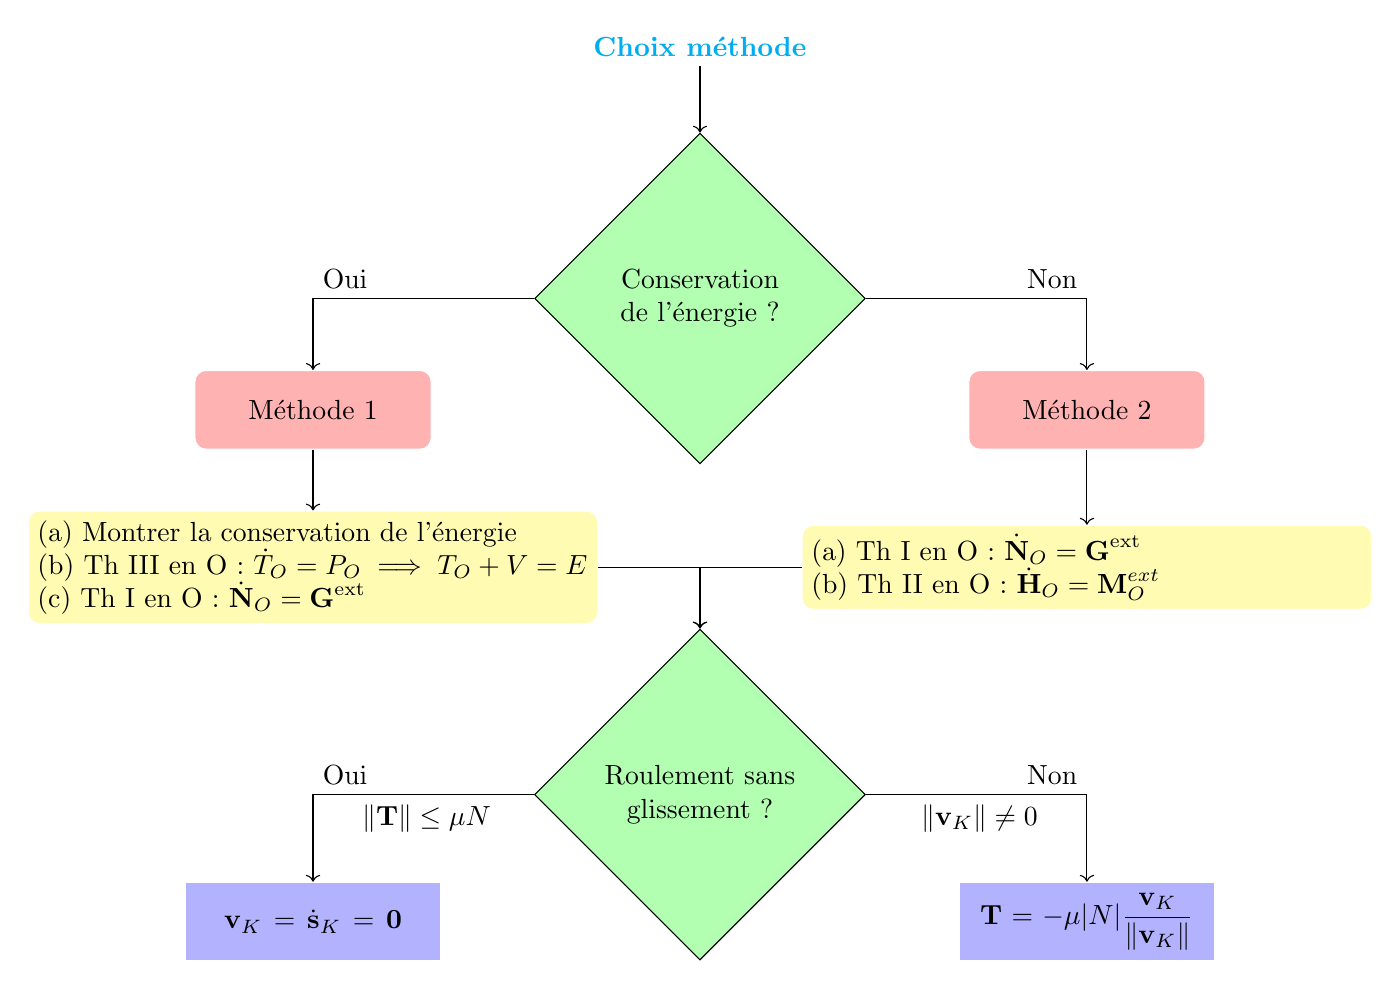
\begin{tikzpicture}[node distance = 2cm]

\node (ChoixMethodes) [vert, text width = 3cm, yshift = -3cm] {Conservation de l'énergie ?};

\node (1) [cyan, above of = ChoixMethodes, yshift = 1.2cm, rounded corners] {\textbf{Choix méthode}};

\node (10) [rouge, below left of = ChoixMethodes, xshift = -3.5cm, draw = white] {Méthode 1};
\node (11) [rouge, below right of = ChoixMethodes, xshift = 3.5cm, draw = white] {Méthode 2};

\node (10a) [rectangle, rounded corners, minimum width = 3cm, minimum height = 1cm, draw = black, fill = yellow!30, xshift = 0cm, below of = 10, text width = 7cm, draw = white] {(a) Montrer la conservation de l'énergie \\ (b) Th III en O : $ \dot{T}_O = \mathpzc{P}_O \implies T_O + V = E $ \\ (c) Th I en O : $ \dot{\textbf{N}}_O = \textbf{G}^{\text{ext}} $};
\node (11a) [rectangle, rounded corners, minimum width = 3cm, minimum height = 1cm, draw = black, fill = yellow!30, xshift = 0cm, below of = 11, text width = 7cm, draw = white] {(a) Th I en O : $ \dot{\textbf{N}}_O = \textbf{G}^{\text{ext}} $ \\ (b) Th II en O : $ \dot{\textbf{H}}_O = \textbf{M}_O^{ext} $};

\node (DecisionGlissement) [vert, below of = 1, text width = 3cm, yshift = -7.5cm] {Roulement sans glissement ?};

\node (2) [bleu, below of = 10, yshift = -4.5cm, draw = white] {$ \textbf{v}_K = \dot{\textbf{s}}_K = \textbf{0} $} ;
\node (3) [bleu, below of = 11, yshift = -4.5cm, draw = white] {$\displaystyle \textbf{T} = - \mu | N | \frac{\textbf{v}_K}{\| \textbf{v}_K \|} $} ;



%% Flèches
\draw[->] (1) -- (ChoixMethodes);
\draw[->] (ChoixMethodes) -| node[anchor = south west]{Oui} (10);
\draw[->] (ChoixMethodes) -| node[anchor = south east]{Non} (11);
\draw[->] (10) -- (10a);
\draw[->] (11) -- (11a);

\draw[->] (10a) -| (DecisionGlissement);
\draw[->] (11a) -| (DecisionGlissement);

\draw[->] (DecisionGlissement) -| node[anchor = south west]{Oui} node[anchor = north west, xshift=0.5cm]{$ \| \textbf{T} \| \leq \mu N $} (2);
\draw[->] (DecisionGlissement) -| node[anchor = south east]{Non} node[anchor = north east, xshift=-0.5cm]{$ \| \textbf{v}_K \| \neq 0 $} (3);

\end{tikzpicture} \end{center}





\begin{tcolorbox}[title=\textcolor{black}{A. Méthode n°1 - Conservation de l'énergie}, colback=white, colframe=sprinen, sharp corners]
\begin{enumerate}
\item Il faut démontrer la conservation de l'énergie (ex : forces appliquées = conservatives \& forces de réaction ne développent pas de puissance)
\item On utilise le \underline{Th. III en \emph{O}} = théorème de l'énergie cinétique en \emph{O} (axes absolus en \emph{O}) : 
\[ \dot{T}_O = \mathpzc{P}_O \]
avec $ T_O + V = E \; \longrightarrow \; $ 1 éq. pour \emph{O}
\item On utilise le \underline{Th. I} = théorème de la quantité de mouvement (axes absolus en \emph{O}) : 
\[ \dot{\textbf{N}}_O = \textbf{G}^{\text{ext}} \]
projeté sur $ \textbf{E}_x $ \& $ \textbf{E}_y $ donne $ \textbf{R}_m $ et $ \textbf{R}_n $ en fonction de $ \theta $.
\end{enumerate}
\end{tcolorbox}





\begin{tcolorbox}[title=B. Méthode n°2 - Fonctionne dans tous les cas, colback=white, colframe=violet!80, sharp corners]
\begin{enumerate}
\item On utilise le \underline{Th. I} = théorème de la quantité de mouvement (axes absolus en \emph{O}) : 
\[ \dot{\textbf{N}}_O = \textbf{G}_{\text{ext}} \]
projeté sur $ \textbf{E}_x $ \& $ \textbf{E}_y $ donne $ \textbf{R}_m $ et $ \textbf{R}_n $ en fonction de $ \theta $.
\item On utilise le \underline{Th. II} = théorème du moment cinétique (axes absolus en O) : 
\[ \dot{\textbf{H}}_O = \textbf{M}_O^{\text{ext}} \]
projeté sur $ \textbf{E}_z \longrightarrow $ 1 éq. si mouvement plan
\end{enumerate}
\end{tcolorbox}

\textcolor{red}{Remarque} : Si le solide décrit un mouvement plan, il y a maximum 3 ddl (degrés de liberté) : Il y a sa propre rotation et le mouvement dans le plan.





















































\newpage










\appendix










\section{Annexes - Mouvement du point matériel}





\subsection{Loi de Newton dans un repère non-inertiel}





Lorsqu'on est dans un repère non-inertiel, une décomposition de l'accélération peut être effectuée : 
\[ \frac{d^2 \textbf{s}}{d t^2} = \underbrace{ \frac{d^2 \textbf{b}}{d t^2} + \dot{\textbf{w}} \wedge \textbf{r} + \textbf{w} \wedge (\textbf{w} \wedge \textbf{r}) }_{\textbf{a}_e} + \underbrace{ 2 \; \textbf{w} \wedge \frac{\delta \textbf{r}}{\delta t} }_{\textbf{a}_c} + \underbrace{ \frac{\delta^2 \textbf{r}}{\delta t^2} }_{\textbf{a}_r} \]
où $ \textbf{a}_e $ est l'accélération d'entraînement, $ \textbf{a}_c $ est l'accélération de Coriolis et $ \textbf{a}_r $ est l'accélération relative.

La \textcolor{red}{\textbf{Loi de Newton}} (équation différentielle vectorielle du mouvement) qui devrait s'écrire : 
\[ \textbf{F} = m \; \ddot{\textbf{s}} \qquad \qquad \qquad \sum \textbf{F}_{\text{extérieures}} = m \; \ddot{\textbf{s}} \]
S'écrit, dans un repère non-inertiel : 
\[ \begin{aligned} m \; \textbf{a}_r = m \frac{\delta^2 \textbf{r}}{\delta t^2} &= \textbf{G} - m \; \textbf{a}_e - m \; \textbf{a}_c \\ &= \textbf{G} - m \Big[ \frac{d^2 \textbf{b}}{d t^2} + \dot{\textbf{w}} \wedge \textbf{r} + \textbf{w} \wedge (\textbf{w} \wedge \textbf{r}) \Big] - m \Big[ 2 \textbf{w} \wedge \frac{\delta \textbf{r}}{\delta t} \Big] \end{aligned} \]






\subsection{Exemple d'oscillateurs harmoniques couplés}





\begin{itemize}




%% Oscillateurs harmoniques couplés
\item Oscillateurs harmoniques couplés : \\
La réponse libre d'oscillateurs harmoniques couplés consiste en une oscillation composite, superposition de plusieurs oscillations périodiques dont les fréquences sont les \emph{fréquences propres} du système. La forme particulière des oscillations harmoniques correspondant à chacune des fréquences propres est appelée \emph{mode de vibration}.

\begin{center}
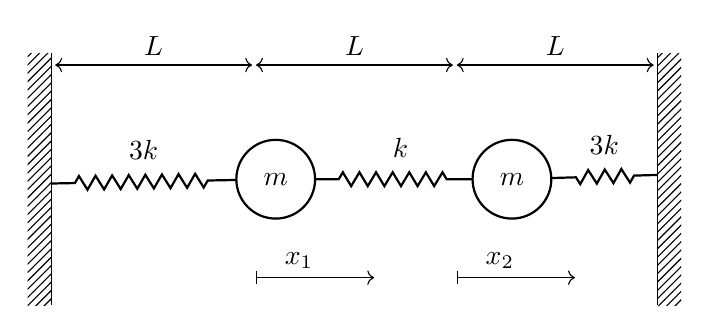
\begin{tikzpicture}[every node/.style={draw,outer sep=0pt,thick}]
\tikzstyle{spring}=[thick,decorate,decoration={zigzag,pre length=0.3cm,post length=0.3cm,segment length=6}]

\tikzstyle{ground}=[fill,pattern=north east lines,draw=none,minimum width=0.75cm,minimum height=0.3cm]


\begin{scope}[xshift=7cm]
\node (M) [circle, thick, minimum size=1cm] {$ m $};
\node (M2) [circle, thick, minimum size=1cm, xshift=3cm] {$ m $};

\node (wall) [ground, rotate=-90, minimum width=3.2cm,yshift=-3cm] {};
\draw (wall.north east) -- (wall.north west);

\node (wall2) [ground, rotate=90, minimum width=3.2cm,yshift=-5cm] {};
\draw (wall2.north east) -- (wall2.north west);

\draw [spring] (wall.70) -- (M) node[pos=.5,left, draw=none, yshift = 0.4cm, xshift=0.3cm]{$ 3 k $};
\draw [spring] (M) -- (M2) node[pos=.5,left, draw=none, yshift = 0.4cm, xshift=0.3cm]{$ k $};
\draw [spring] (wall2.70) -- (M2) node[pos=.5,left, draw=none, yshift = 0.4cm, xshift=0.3cm]{$ 3 k $};

\draw [<->, xshift = -2.8cm, yshift = 1.45cm] (0,0) -- (2.5cm,0) node[anchor=south, draw=none, xshift=-1.25cm]{$ L $};
\draw [<->, xshift = -0.25cm, yshift = 1.45cm] (0,0) -- (2.5cm,0) node[anchor=south, draw=none, xshift=-1.25cm]{$ L $};
\draw [<->, xshift = 2.3cm, yshift = 1.45cm] (0,0) -- (2.5cm,0) node[anchor=south, draw=none, xshift=-1.25cm]{$ L $};

\draw [|->, xshift = -0.25cm, yshift = -1.25cm] (0,0) -- (1.5cm,0) node[anchor=south west, draw=none, xshift=-1.25cm]{$ x_1 $};
\draw [|->, xshift = 2.3cm, yshift = -1.25cm] (0,0) -- (1.5cm,0) node[anchor=south west, draw=none, xshift=-1.25cm]{$ x_2 $};

\end{scope}
\end{tikzpicture}
\end{center}

Si on place les axes à la longueur naturelle des ressorts, les équations du mouvement s'écrivent : 
\[ \begin{aligned} m \ddot{x}_1 + 3 k x_1 - k (x_2 - x_1) &= 0 \\ m \ddot{x}_2 + 3 k x_2 - k (x_1 - x_2) &= 0 \end{aligned} \]
On découple ces équations en posant : 
\[ \begin{aligned} X_1 &= x_1 + x_2 \\ X_2 &= x_1 - x_2 \end{aligned} \qquad \qquad \begin{aligned} 2 x_1 &= X_1 + X_2 \\ 2 x_2 &= X_1 - X_2 \end{aligned} \]
D'un point de vue physique, $ X_1 $ décrit le déplacement du centre d'inertie du système. \\
On obtient alors : 
\[ \begin{aligned} m \ddot{X}_1 + 3 k X_1 &= 0 \\ m \ddot{X}_2 + 5 k X_2 &= 0 \end{aligned} \qquad \implies \qquad
\begin{aligned} X_1 &= C_1 \cos (\sqrt{3} \; \omega_0 t + \varphi_1) \\ X_2 &= C_2 \cos (\sqrt{5} \; \omega_0 t + \varphi_2) \end{aligned} \]
où $ \omega_0^2 = k/m $. Les fréquences propres du systèmes sont donc $ \omega_I = \sqrt{3} \; \omega_0 $ et $ \omega_{II} = \sqrt{5} \; \omega_0 $.
\begin{center} \begin{tabular}{lll}
Si $ x_1 = x_2 $, & les 2 points matériels oscillent en phase & (fréquence $ = \omega_I $) \cr
Si $ x_1 = - x_2 $, & les 2 points matériels oscillent en opposition de phase & (fréquence $ = \omega_{II} $)
\end{tabular} \end{center}





%% Oscillateurs harmoniques couplés - forçage périodique
\item Dans le cas envisagé, si on applique une force \textbf{F} au premier point matériel du système telle que $ F = m L \Omega^2 \cos \omega t $, on a : 
\[ \begin{aligned} m \ddot{x}_1 + 3 k x_1 - k (x_2 - x_1) &= m L \Omega^2 \cos \omega t \\ m \ddot{x}_2 + 3 k x_2 - k (x_1 - x_2) &= 0 \end{aligned} \qquad \implies \qquad 
\begin{aligned} m \ddot{X}_1 + 3 k X_1 &= m L \Omega^2 \cos \omega t \\ m \ddot{X}_2 + 5 k X_2 &= m L \Omega^2 \cos \omega t \end{aligned} \]
On peut donc étudier séparément la réponse de chacun des modes propres soumis à une force excitatrice. On dit de cette force s'appliquant à un mode particulier qu'elle est la \emph{projection de la force appliquée dans la base des modes propres}. \\
Et si $ x_1 = x_2 = 0 \; ; \; \dot{x}_1 = \dot{x}_2 = 0 $, on a : 
\[ X_1 = \frac{L \Omega^2}{\omega_I^2 - \omega^2} (\cos \omega t - \cos \omega_I t) \qquad \qquad X_2 = \frac{L \Omega^2}{\omega_{II}^2 - \omega^2} (\cos \omega t - \cos \omega_{II} t) \]
Si $ \omega = \omega_I $ ou si $ \omega = \omega_{II} $, alors il y a résonance et la solution ci-dessus n'est plus correcte. Par exemple, si $ \omega = \omega_I $, on a : 
\[ X_1 = \frac{L \Omega^2}{2 \omega_I} t \sin \omega_I t \]





%% Note sur les modes propres
\item Note sur les modes propres : \\
Un mode normal ou mode propre d'oscillation est une forme de mouvement dans laquelle toutes les parties du système se déplacent sinusoïdalement avec la même fréquence naturelle de vibration associée au mode. \\
Le nombre de modes normaux est égal à celui des degrés de liberté du système.

Le mouvement général d'un système est la superposition de ses modes normaux. Les modes sont normaux dans le sens qu'ils se déplacent indépendamment les uns des autres, une excitation d'un des modes ne cause jamais le mouvement d'un autre mode. En termes mathématiques, les modes sont orthogonaux.






\end{itemize}










\subsection{Stabilité et dérivées}





\begin{itemize}





%% Rappel : extrema d'une fonction
\item Rappel : Extrema d'une fonction : \\
Si \emph{f} est une fonction réelle $ n + 1 $ fois continûment dérivable sur $ ]a, b[ $, si $ f'(c) = 0 $ en un point $ c \in \; ]a, b[ $ et si la première dérivée non-nulle en \emph{c} est $ f^{(n)} (c) $, alors : 
\begin{itemize}
\item[--] \emph{c} est un maximum local si \emph{n} est pair et $ f^{(n)}(c) < 0 $.
\item[--] \emph{c} est un minimum local si \emph{n} est pair et $ f^{(n)}(c) > 0 $.
\item[--] \emph{c} est un point d'inflexion à tangente horizontale si \emph{n} est pair.
\end{itemize}





%% Types d'équilibre
\item Pour rappel, on a 4 types "d'équilibres" : Stable, Instable, Marginalement Stable, Faiblement Instable. \\
Et par exemple, si on a une équation différentielle linéaire à coefficients constants dont on veut connaître la stabilité : 

\begin{center} \begin{tabular}{p{6cm}|p{6cm}}

    Racines du polynôme caractéristique : $ z_1 = a_1 + i b_1 \; \; \text{et} \; \; z_2 = a_2 + i b_2 $ & Stabilité : méthode des perturbations infinitésimales (éq. linéaire)
    \\ & \\ \hline & \\

    $ a_1 < 0 $ et $ a_2 < 0 $ & Équilibre \textbf{stable}
    \[ x(t) = C_1 e^{- x t} + C_2 e^{- y t} \] \\

    Si $ a_1 > 0 $ ou $ a_2 > 0 $ & Équilibre \textbf{instable}
    \[ x(t) = C'_1 e^{\alpha t} + C'_2 e^{- \alpha t} = C_1 \text{ sh } \alpha t + C_2 \text{ ch } \alpha t \] \\

    $ a_1 < 0, \; a_2 = 0 $ \; ou \; $ a_1 = 0, \; a_2 < 0  $ \; \danger avec $ k = 0 $ \quad (k = multiplicité) & Équilibre \textbf{marginalement stable}, \[ x(t) = C'_1 e^{i \alpha t} + C'_2 e^{- i \alpha t} \; = C_1 \sin \alpha t + C_2 \cos \alpha t \] \\

    $ z_1 = z_2 = 0 $ \qquad ($ k \neq 0 $) & Équilibre \textbf{faiblement instable} \[ x(t) = A t + B \]

\end{tabular} \end{center}




\end{itemize}










\newpage










\section{Annexes - Mouvement du solide}





\subsection{Intégrer sur des volumes/surfaces}





\begin{itemize}





%% Calcul d'aire et volume
\item Calcul d'aire et volume : Une aire se calcule avec la formule $\displaystyle A = \iint_\Omega 1 \; d x \; d y = \iint_\Omega d x \; d y $ \\ et le volume avec la formule $\displaystyle V = \iiint_\Omega 1 \; d x \; d y \; d z = \iiint_\Omega \; d x \; d y \; d z $.






%% Réduction des intégrales dans R^n
\item Réduction des intégrales dans $ \mathbb{R}^n $ : 

\begin{center}
\includegraphics[width=0.5\textwidth]{tetraedre.PNG}
\end{center}

Calculer le volume du tétraèdre : 
\begin{align*}
V = \iiint_\Omega d x \; d y \; d z &= \int_0^a d x \iint_{\Sigma (x)} d y \; d z \\
 &= \int_0^a d x \int_0^{b - \frac{b x}{a}} d y \int_0^{c (1 - \frac{y}{b} - \frac{x}{a})} d z \\
 &= \int_0^a d x \int_0^{b - \frac{b x}{a}} c \bigg( 1 - \frac{y}{b} - \frac{x}{a} \bigg) d y \\
 &= c \int_0^a \bigg[ y - \frac{y^2}{2 b} - \frac{x y}{a} \bigg]_{y=0}^{y=b-\frac{b x}{a}} d x \\
 &= c \int_0^a \bigg( \frac{b x^2}{2 a^2} - \frac{b x}{a} + \frac{b}{2} \bigg) d x \\
 &= \frac{a b c}{6}
\end{align*}





%% Systèmes de coordonnées
\item Systèmes de coordonnées : 
\begin{center} \includegraphics[width=9cm]{dAdV.png} \end{center}
\begin{center} \begin{tabular}{|c|ccc|} \hline
& Cartésien & Cylindrique & Sphérique \\
& $ f(x, y, z) $ & $ f(r, \theta, z) $ & $ f(\rho, \theta, \phi) $ \\ \hline
$ x $ & $ x $ & $ r \cos \theta $ & $ \rho \cos \theta \sin \phi $ \\
$ y $ & $ y $ & $ r \sin \theta $ & $ \rho \sin \theta \sin \phi $ \\
$ z $ & $ z $ & $ z $ & $ \rho \cos \phi $ \\
$ r $ & $ \sqrt{x^2 + y^2} $ & $ r $ & $ \rho \sin \phi $ \\
$ \theta $ & $\displaystyle \tan^{-1} \bigg( \frac{y}{x} \bigg) $ & $ \theta $ & $ \theta $ \\
$ \rho $ & $ \sqrt{x^2 + y^2 + z^2} $ & $ \sqrt{r^2 + z^2} $ & $ \rho $ \\
$ \phi $ & $\displaystyle \tan^{-1} \bigg( \frac{\sqrt{x^2 + y^2}}{z} \bigg) $ & $\displaystyle \tan^{-1} \bigg( \frac{r}{z} \bigg) $ & $ \phi $ \\ \hline
\end{tabular} \end{center}





%% Aire d'une surface courbe
\item Aire d'une surface courbe : On définit l'aire d'une surface courbe régulière $ \Sigma $ par la formule : 
\[ S = \iint_\Sigma d \sigma = \iint_\Omega \bigg\| \frac{d \textbf{s}}{d u} \wedge \frac{d \textbf{s}}{d v} \bigg\| \; d u \; d v \]
si cette intégrale existe, c-à-d si : 
\[  \bigg\| \frac{d \textbf{s}}{d u} \wedge \frac{d \textbf{s}}{d v} \bigg\| \in \mathbb{L}_1(\Omega) \]
avec : $ \textbf{s} = x \; \textbf{e}_1 + y \; \textbf{e}_2 + z \; \textbf{e}_3 $.





%% Surface de révolution
\item Surface de révolution : Si une surface est engendrée par la rotation d'une courbe plane $ y = f(x) \geq 0 $ autour de l'axe OX, on peut introduire le paramétrage, 
\[ \textbf{s}(x, \theta) = x \textbf{e}_x + f(x) \cos(\theta) \textbf{e}_y + f(x) \sin(\theta) \textbf{e}_z, \qquad x \in \; ]a, b[, \; \theta \in \; ]0, 2 \pi[ \]
Et on a donc la formule pour la surface : 
\[ S = \iint_\Sigma d \sigma = 2 \pi \int_a^b f(x) \sqrt{1 + \big[ f'(x) \big]^2} \; d x \]





%% Surface d'un tore
\item Surface d'un tore ($ R > a $) : 

\begin{center}
  \makebox[\textwidth]{
    \includegraphics[width=0.35\paperwidth]{tore.PNG}
    \includegraphics[width=0.2\paperwidth]{tore2.jpg}
}
\end{center}

En utilisant les vecteurs unitaires des coordonnées cylindriques, la surface est décrite par : 
\[ \textbf{s}(\theta, \phi) = \big( R + a \cos \phi \big) \; \textbf{e}_r(\theta) + a \sin \theta \; \textbf{e}_z, \qquad \theta \in \; ]0, 2 \pi[, \; \; \phi \in \; ]0, 2 \pi[ \]
de sorte que 

\begin{align*}
d \sigma &= \Big\| \big( R + a \cos \phi \big) \; \textbf{e}_\theta \wedge \big( - a \sin \phi \; \textbf{e}_r + a \cos \phi \; \textbf{e}_z \big) \Big\| \; d \theta \; d \phi \cr
&= \big( R + a \cos \phi \big) a \; d \theta \; d \phi
\end{align*}
Il vient dés lors 
\[ S = \int_0^{2 \pi} d \theta \int_0^{2 \pi} \big( R + a \cos \phi \big) a \; d \phi = 4 \pi^2 R a \]






\end{itemize}





\subsection{Exemple de calcul du tenseur d'inertie d'une sphère en coordonnées cylindriques}





Exemple : Calcul de $ J_3 $ en coordonnées cylindriques ($ \textbf{J}_C = J \; \textbf{I} $).

\begin{center} 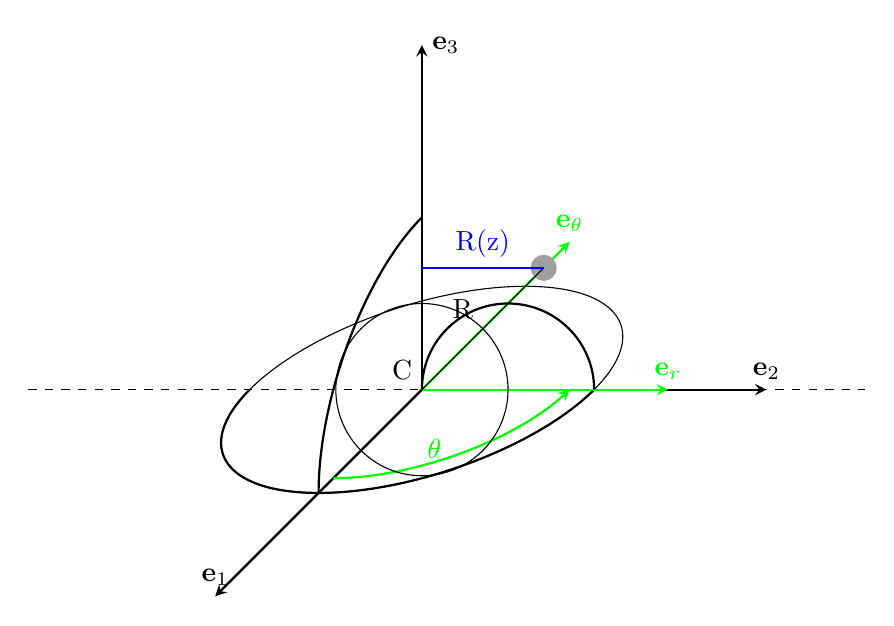
\begin{tikzpicture}[x=0.5cm,y=0.5cm,z=0.3cm,>=stealth, scale=1.25]

% The axes
\draw[->, thick] (xyz cs:x=0) -- (xyz cs:x=7) node[above] {$\textbf{e}_2$};
\draw[->, thick] (xyz cs:y=0) -- (xyz cs:y=7) node[right] {$\textbf{e}_3$};
\draw[->, thick] (xyz cs:z=0) -- (xyz cs:z=-7) node[above] {$\textbf{e}_1$};

% Dashed line
\draw[-, dashed] (xyz cs:x=-8) -- (xyz cs:x=9) ;

% Define planes
[x={(10cm,10cm)}, y={(-3cm,-3cm)}, z={(10cm,10cm)}, scale=0.2]
\tikzset{Hplane/.style={canvas is zx plane at y=#1}}
\tikzset{Vplane/.style={canvas is xy plane at z=#1}}
\tikzset{V2plane/.style={canvas is yz plane at x=#1}}

% Horizontal plane - Hplane
\begin{scope}[Hplane=0]
\draw (0,0) node[anchor=south east]{C} circle[radius=3.5cm] ;
\draw [-, thick] (0,3.5) arc (90:270:3.5cm) ;
\draw[->, thick, green] (xyz cs:x=0) -- (xyz cs:x=5) node[above] {$\textbf{e}_\theta$};
\draw[->, thick, green] (xyz cs:y=0) -- (xyz cs:y=5) node[above] {$\textbf{e}_r$};
\draw [->, thick, green] (-3,0) arc (180:90:3cm) node[anchor=south east, xshift=-1.5cm, yshift=-1cm]{$ \theta $} ;
\end{scope}

% In front of me (Vertical) plane - Vplane
\begin{scope}[Vplane=0]
\draw (0,0) circle[radius=1.75cm] ;
\draw [-, thick] (3.5,0) arc (0:180:1.75cm) ;
\node (boule) at (2.475,2.475) [circle, xshift = 0cm, yshift = 0cm, fill=gray!75] {};
\draw[-] (0,0) -- node[anchor = south east]{R} (2.475,2.475) ;
\draw[-, blue, thick] (0,2.475) -- node[anchor = south]{R(z)} (2.475,2.475) ;
\end{scope}

% Other vertical plane - V2plane
\begin{scope}[V2plane=0]
\draw[-,thick] (0,-3.5) arc (270:360:3.5cm) ;
\end{scope}

\end{tikzpicture} \end{center}

$\displaystyle J = J_3 = \int_{\text{sphère}} ( x_1^2 + x_2^2 ) \; d m $, \qquad avec $ d m = \rho \; d x_1 ; d x_2 \; d x_3 $ \\
$\displaystyle J = \rho \int_0^{2 \pi} d \theta \int_{-R}^R d z \int_0^{R(z) = \sqrt{R^2 - z^2}} \big( (r \cos \theta)^2 + (r \sin \theta)^2 \big) \underbrace{r}_{\text{Jacobien}} d r = \frac{16}{15} R^5 $ \\
$\displaystyle \rho =  \frac{m}{\frac{4}{3} \pi R^3} \implies J = \frac{2}{5} m R^2 $





\subsection{Théorèmes généraux en dynamique du solide}






%% Dynamique du solide : Théorème généraux
Un solide indéformable peut avoir jusqu'à six degrés de liberté (3 de translation et 3 de rotation), pour déterminer le mouvement d'un solide, on a donc affaire à 6 inconnues.
\[
\left.\begin{aligned}
\text{ Th. I } \quad & m \ddot{\textbf{c}} = \textbf{G} \quad & 3 \text{ équations } \\
\text{ Th. II } \quad & \dot{\textbf{H}}_O = \textbf{M}_O \quad & 3 \text{ équations } \\
\text{ Th. II}_C \quad & \dot{\textbf{H}}_C = \textbf{M}_C \quad & 3 \text{ équations } \\
\text{ Th. III } \quad & \dot{T}_O = \mathpzc{P}_O \quad & 1 \text{ équation } \\
\text{ Th. III}_C \quad & \dot{T}_C = \mathpzc{P}_C \quad & 1 \text{ équation }
\end{aligned}\right\rbrace \qquad \implies 11 \text{ équations }
\]





\subsection{Exemple : Déterminer la relation entre les coordonnées généralisés exprimant le roulement sans glissement}





%% Roulement sans glissement
Roulement sans glissement : 
\begin{center} \begin{tabular}{M{8cm}M{5cm}}
\includegraphics[width=0.45\textwidth]{Solides3.PNG}
&
\[ \begin{aligned}
\textbf{s}_p &= x \textbf{e}_x + R \textbf{e}_y + R \textbf{e}_r \\
\dot{\textbf{s}}_p &= \dot{x} \textbf{e}_x + R \dot{\theta} \textbf{e}_\theta
\end{aligned} \]
\[ \fbox{$ \; \dot{x} + R \dot{\theta} = 0 \; $} \]
\end{tabular} \end{center}













\newpage













\section{Q.III Janvier 2017}





\subsection{Application de la méthode générale}





\begin{center} \includegraphics[width=0.75\textwidth]{Q3Jan2017.PNG} \end{center}





\begin{enumerate}

%% 1
\item \textcolor{red}{Type de système} et \textcolor{orange}{caractéristiques} : 
\begin{itemize}
    \item Roues identiques (rayon \emph{a}),
    \item reliées par un axe horizontal (rayon \emph{b}, avec $ b < a $),
    \item sur un plan incliné (angle $ \alpha $ par rapport à l'horizontale),
    \item système de masse \emph{m},
    \item coefficient de frottement $ \mu $,
    \item centre d'inertie ( \emph{C} ) situé au centre géométrique,
    \item moment central d'inertie (rotation axe horizontal) $ = \Gamma $.
    \item Une corde inextensible (masse négligeable) se déroule sans frottement et est attachée à l'axe horizontal (voir dessin ci-dessus).
\end{itemize}

%% 2
\item Le système roule sans glisser parallèlement au plan. Le mouvement du système est étudié comme un \textcolor{red}{mouvement plan}. \\
Puisque le solide est en mouvement plan, il possède 3 degrés de libertés \emph{au maximum}. Le contact entre le système et le plan, et la condition de roulement sans glissement donnent 2 contraintes cinématiques, ce qui fait que le système n'a qu'un seul degré de liberté (\textcolor{orange}{1 ddl}).

%% 3
\item \textcolor{red}{Systèmes d'axes} : 
\begin{enumerate}
    \item On place un \textcolor{orange}{repère absolu} : O, $ \textbf{E}_x $, $ \textbf{E}_y $, $ \textbf{E}_z $, ici avec O au pied du plan incliné, $ \textbf{E}_x $ parallèle au plan (angle $ \alpha $ avec l'horizontale), $ \textbf{E}_y \perp \textbf{E}_x $ et $ \textbf{E}_z $ perpendiculaire au plan contenant le mouvement ($ \textbf{E}_z $ pointe \emph{en-dehors} de la feuille).
    \item On n'a pas besoin d'ajouter un système d'axe ici car le repère absolu est suffisant. On va juste introduire les \textcolor{red}{coordonnées généralisées} \emph{x} (décrit le mouvement de \emph{C}) et $ \theta $ (décrit la rotation du solide autour de \emph{C}).
\end{enumerate}

\begin{center} \includegraphics[width=0.55\textwidth]{Q3Jan2017-2.PNG} \end{center}

%% 4
\item Les \textcolor{orange}{forces extérieures} appliquées au système sont : 
\begin{itemize}
    \item La force de pesanteur $ m \textbf{g} $, force extérieure conservative appliquée en \emph{C} et dirigée verticalement vers le bas.
    \item La force de liaison $ \textbf{R} = N \textbf{E}_y + T \textbf{E}_x $ appliquée en \emph{K}, de direction inconnue;
    \item  La force extérieure $ \textbf{F}(t) $ appliquée en l’extrémité de la corde et parallèle au plan incliné.
\end{itemize}


\end{enumerate}





\begin{center} \textbf{Une fois que l’on a fait ceci, on doit choisir la méthode que l’on va utiliser en fonction du problème.} \end{center}





\subsection{Application de la méthode 2}





On va suivre la méthode n°2 qui fonctionne dans tous les cas.
\begin{center} 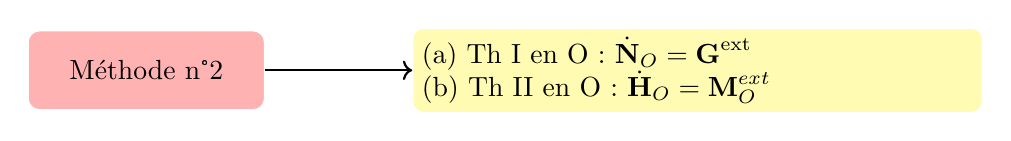
\begin{tikzpicture}
\node (2) [rouge, draw = white] {Méthode n°2} ;

\node (2a) [rectangle, rounded corners, minimum width = 3cm, minimum height = 1cm, draw = black, fill = yellow!30, xshift = 0cm, xshift=7cm, text width = 7cm, draw = white] {(a) Th I en O : $ \dot{\textbf{N}}_O = \textbf{G}^{\text{ext}} $ \\ (b) Th II en O : $ \dot{\textbf{H}}_O = \textbf{M}_O^{ext} $} ;

\draw[thick, ->] (2) -- (2a) ;
\end{tikzpicture} \end{center}

Pourquoi la méthode 2 ? Parce que le roulement sans glissement implique qu'il y ait une force de frottement qui développe inévitablement une puissance et il n'y a donc pas de conservation de l'énergie, condition nécessaire pour utiliser la méthode 1.





\begin{siderules}
\begin{enumerate}[(a)]

%% (a)
\item $\displaystyle \dot{\textbf{N}}_O = \textbf{G}^{\text{ext}} \implies m \ddot{x} \; \textbf{E}_x = m \; \textbf{g} + \textbf{R} + \textbf{F} $ \\
Quand on projette cette équation sur les axes $ \textbf{E}_x $ et $ \textbf{E}_y $, on obtient : 
    \begin{equation} %% Équation n°1
        m \ddot{x} = - m g \sin \alpha + F + T
    \end{equation}
    \begin{equation} %% Équation n°2
        0 = - m g \cos \alpha + N
    \end{equation}

%% (b)
\item Plutôt que d'utiliser le théorème : $ \dot{\textbf{H}}_O = \textbf{M}_O^{\text{ext}} $, on va utiliser : $ \dot{\textbf{H}}_C = \textbf{M}_C^{\text{ext}} $ dans un système d'axes en \emph{C} parallèles aux axes inertiaux. \\
Puisque : $ \textbf{H}_C = \textbf{J}_C \cdot \boldsymbol{\omega} = \Gamma \dot{\theta} \; \textbf{E}_z $, \\
$ \textbf{M}_C = - a \; \textbf{E}_y \wedge \textbf{R} + b \; \textbf{E}_y \wedge \textbf{F} $, on a : 
\[ 
\begin{aligned}
\dot{\textbf{H}}_C = \textbf{M}_C \implies \Gamma \ddot{\theta} \; \textbf{E}_z &= - a \; \textbf{E}_y \wedge \textbf{R} + b \; \textbf{E}_y \wedge \textbf{F} \\
&= a T \; \textbf{E}_z - b F \; \textbf{E}_z
\end{aligned}
\]
Si on fait un produit scalaire ($ \cdot \; \textbf{E}_z $) sur les 2 membres de l'équation, on a : 
    \begin{equation}
        \Gamma \ddot{\theta} = a T - b F
    \end{equation}
\end{enumerate}
\end{siderules}





\subsection{Relation entre les coordonnées généralisées exprimant le roulement sans glissement}





Le roulement sans glissement se traduit par la condition : 
\[ \dot{\textbf{s}}_K^{\text{Syst}} = \dot{\textbf{s}}_K^{\text{Plan}} \]
Puisque le plan incliné est immobile, on a : $ \dot{\textbf{s}}_K^{\text{Syst}} = \dot{\textbf{s}}_K^{\text{Plan}} = \textbf{0} $. La vitesse d’un point matériel \emph{P} quelconque du système étudié est donnée par (avec \textbf{c} la position de \emph{C}) : 
\[ \dot{\textbf{s}}_P = \dot{\textbf{c}} + \boldsymbol{\omega} \wedge \textbf{CP} \]
Et la vitesse de \emph{K} : 
\[ \begin{aligned}
\dot{\textbf{s}}_K &= \dot{\textbf{c}} + \boldsymbol{\omega} \wedge \textbf{CK} \\
&= \dot{x} \; \textbf{E}_x + \dot{\theta} \; \textbf{E}_z \wedge (- a) \; \textbf{E}_y \\
&= (\dot{x} + a \dot{\theta}) \; \textbf{E}_x
\end{aligned} \]
ainsi, la condition de roulement sans glissement est donnée par : $ \dot{x} + a \; \dot{\theta} = 0 $.





\subsection{Sous-Questions Supplémentaires}





\begin{enumerate}[i.]
\item[vi.] Déterminer l'intensité de \textbf{F} ($ = F_0 $) pour maintenir le système au repos. (1)
\item[vii.] Déterminer la valeur max de l’inclinaison du plan permettant l’équilibre identifié en vi. (2)
\item[viii.] Déterminer l’accélération de \emph{C} en fonction de \emph{F} lorsque : $ F(t) = \| \textbf{F}(t) \| > F_0 $. (3)
\item[ix.] Montrez qu’on peut communiquer un roulement sans glissement avec une accélération arbitrairement grande pour autant que : $\displaystyle \tan \alpha \leq \mu \bigg( 1 + \frac{m a^2}{\Gamma} \bigg) $, à condition de choisir judicieusement le rayon \emph{b} de l’axe horizontal sur lequel s’enroule la corde. (4)
\end{enumerate}





\begin{enumerate}[(1)]

\item Au repos, les 3 équations deviennent : $\displaystyle \begin{cases}
0 = - m g \sin \alpha + F + T \\
0 = - m g \cos \alpha + N \\
0 = a T - b F
\end{cases} \quad \implies F_0 = \frac{m g a \sin \alpha}{a + b} $

\item En \emph{K}, on a : $\displaystyle \begin{cases}
N_0 = m g \cos \alpha \\
\displaystyle T_0 = \frac{m g b \sin \alpha}{a + b}
\end{cases} $. Cette solution n'est acceptable que si on respecte les conditions de roulement sans glissement, notamment : $ |T_0| \leq \mu |N_0| \implies m g b \sin \alpha \leq (a + b) \mu m g \cos \alpha $ \\
$\displaystyle \implies \tan \alpha \leq \frac{a + b}{b} \mu $.

\item On utilise les éq. (1), (2) et (3) et la cond. de roulement sans glissement pour isoler \emph{T} et \emph{N} et trouver : 
\[ \ddot{x} = \frac{F a (a + b) - m g a^2 \sin \alpha}{\Gamma + m a^2} \]
On remarque que le système possède une accélération positive vers le haut du plan incliné ($ \ddot{x} > 0 $) si : 
\[ F > F_0 = \frac{m g a \sin \alpha}{a + b} \]

\item Il y a 2 conditions pour un roulement sans glissement : $ \textbf{v}_K = \textbf{0} $ et $ |T| \leq \mu |N| $. La deuxième condition est plus intéressante puisqu'elle implique des forces. Une idée est donc d'isoler \emph{T} et \emph{N}. On trouve pour \emph{T} : $\displaystyle T = \frac{m g \Gamma \sin \alpha - (\Gamma - m a b) F}{\Gamma + m a^2} $, qui est indépendant de \emph{F} lorsque : $\displaystyle b = \frac{\Gamma}{m a} $. \\
On continue le raisonnement et on trouve : 
\[ \tan \alpha \leq \mu \bigg( 1 + \frac{m a^2}{\Gamma} \bigg) \]
comme prévu.

\end{enumerate}












































\end{document}
